% Compile from repo root: xelatex -interaction=nonstopmode production/tikz-preview-ch11.tex
\documentclass[UTF8,fontset=fandol,10pt]{ctexart}
\usepackage{graphicx}
% SPDX-License-Identifier: MIT
\usepackage{fontspec}
\setmainfont{texgyrepagella-regular.otf}[
  BoldFont=texgyrepagella-bold.otf,
  ItalicFont=texgyrepagella-italic.otf,
  BoldItalicFont=texgyrepagella-bolditalic.otf]
\setsansfont{texgyreheros-regular.otf}[
  BoldFont=texgyreheros-bold.otf,
  ItalicFont=texgyreheros-italic.otf,
  BoldItalicFont=texgyreheros-bolditalic.otf]
\setmonofont{lmmono10-regular.otf}[Scale=MatchLowercase]
\usepackage[paperwidth=170mm,paperheight=240mm,inner=20mm,outer=18mm,top=20mm,bottom=22mm,headheight=15pt]{geometry}
\usepackage{graphicx,booktabs,tabularx,longtable,array}
\usepackage{amsmath,amssymb}
\usepackage{enumitem}
\usepackage{xcolor}
\definecolor{BookTeal}{HTML}{176C68}
\definecolor{BookInk}{HTML}{23363E}
\definecolor{BookRule}{HTML}{C8D6D6}
\definecolor{BookPale}{HTML}{F1F6F5}
\usepackage{tikz}
\usetikzlibrary{arrows.meta,positioning,shapes.geometric,shapes.misc,fit,backgrounds,calc,matrix}
\usepackage{rotating}
\usepackage{pdfpages}
\usepackage{fvextra}
\DefineVerbatimEnvironment{Prompt}{Verbatim}{fontsize=\small,breaklines=true,breakanywhere=true,frame=single,rulecolor=\color{BookRule},framesep=2mm}
\usepackage{caption}
\captionsetup{font=small,labelfont=bf,labelsep=period}
\usepackage{fancyhdr}
\pagestyle{fancy}
\fancyhf{}
\fancyhead[LE,RO]{\small\thepage}
\fancyhead[LO,RE]{\small\nouppercase{\leftmark}}
\renewcommand{\headrulewidth}{0.3pt}
\usepackage{xurl}
\usepackage[unicode,hypertexnames=false,colorlinks=true,linkcolor=BookTeal,urlcolor=BookTeal,citecolor=BookTeal,breaklinks=true]{hyperref}
\usepackage{bookmark}
\setcounter{tocdepth}{1}
\setcounter{secnumdepth}{1}
\let\cleardoublepage\clearpage
\setlist{nosep,leftmargin=1.8em}
\renewcommand{\arraystretch}{1.25}
\setlength{\parskip}{0.3em}
\setlength{\emergencystretch}{2em}
\newcommand{\bookversion}{0.1.0}
\newcommand{\bookdate}{2026-10-29}
\newcommand{\scidraw}{SciDraw AI}
% Drawn marks: the book fonts lack U+2713/U+2715.
\newcommand{\bookcheck}{\tikz[x=1em,y=1em,baseline=-0.1em,line width=0.12em,line cap=round,line join=round]\draw[color=.] (0,0.3)--(0.28,0)--(0.75,0.7);}
\newcommand{\bookcross}{\tikz[x=1em,y=1em,baseline=-0.1em,line width=0.12em,line cap=round]{\draw[color=.] (0,0)--(0.6,0.65);\draw[color=.] (0,0.65)--(0.6,0);}}
% Circled numbers and the inhibition sign are missing from the book fonts; draw them.
\usepackage{newunicodechar}
\newcommand{\bookcirc}[1]{\tikz[baseline=(n.base)]\node[circle,draw,inner sep=0.5pt,minimum size=1.05em,font=\sffamily\scriptsize] (n) {#1};}
\newcommand{\bookcircfill}[1]{\tikz[baseline=(n.base)]\node[circle,fill,inner sep=0.5pt,minimum size=1.05em,font=\sffamily\scriptsize\bfseries,text=white] (n) {#1};}
\newunicodechar{①}{\bookcirc{1}}
\newunicodechar{②}{\bookcirc{2}}
\newunicodechar{③}{\bookcirc{3}}
\newunicodechar{④}{\bookcirc{4}}
\newunicodechar{⑤}{\bookcirc{5}}
\newunicodechar{⑥}{\bookcirc{6}}
\newunicodechar{⑦}{\bookcirc{7}}
\newunicodechar{⑧}{\bookcirc{8}}
\newunicodechar{⑨}{\bookcirc{9}}
\newunicodechar{⑩}{\bookcirc{10}}
\newunicodechar{⑪}{\bookcirc{11}}
\newunicodechar{⑫}{\bookcirc{12}}
\newunicodechar{⑬}{\bookcirc{13}}
\newunicodechar{❶}{\bookcircfill{1}}
\newunicodechar{❷}{\bookcircfill{2}}
\newunicodechar{❸}{\bookcircfill{3}}
\newunicodechar{❹}{\bookcircfill{4}}
\newunicodechar{❺}{\bookcircfill{5}}
\newunicodechar{❻}{\bookcircfill{6}}
\newunicodechar{❼}{\bookcircfill{7}}
\newunicodechar{⊣}{\ensuremath{\dashv}}
\providecommand{\sdbase}{https://sci-draw.com}
\newcommand{\sdtool}[1]{\href{\sdbase/#1}{\texttt{/#1}}}
\newcommand{\bookrepo}{https://github.com/TopLocalAI/ai-scientific-figures-book}
\newenvironment{BookNote}{\begin{quote}\small\color{BookInk}}{\end{quote}}
\newcolumntype{Y}{>{\raggedright\arraybackslash}X}
\newcommand{\workflowfigure}[2]{%
  \begin{figure}[htbp]\centering
  \input{figures/workflow-#1.tex}
  \caption{#2}\label{fig:workflow}
  \end{figure}}
\newcommand{\pairedfigure}[2]{%
  \begin{figure}[htbp]\centering
  \includegraphics[width=\linewidth]{figures/paired-comparison-#1.pdf}
  \caption{#2}\label{fig:paired}
  \end{figure}}

\makeatletter
\let\ChEleven@defcolor\definecolor
\renewcommand{\definecolor}[3]{%
  \@ifundefined{color@#1}{\ChEleven@defcolor{#1}{#2}{#3}}{}%
}
\makeatother
\setlength{\parindent}{0pt}
\begin{document}
\section*{FIG ch11-01 three levels (zh)}
% FIG ch11-01 three levels (Chinese)
\usetikzlibrary{arrows.meta,positioning,calc}
\begin{tikzpicture}[x=\linewidth/100,y=\linewidth/100]
\begin{scope}[
  font=\sffamily\small,
  level/.style={
    draw=BookRule, line width=0.5pt, rounded corners=2pt,
    minimum width=52mm, minimum height=11mm, align=left, inner sep=4pt,
    text width=50mm, anchor=west,
  },
  qbox/.style={
    draw=BookRule, fill=BookPale!40, rounded corners=2pt,
    align=center, inner sep=3pt, text width=22mm, font=\scriptsize,
  },
]
  \node[
    draw=BookTeal, line width=0.7pt, fill=white, rounded corners=3pt,
    align=center, inner sep=5pt, text width=24mm, font=\small,
  ] (bubble) at (8,42) {再好看一点};
  \draw[BookInk!55, dashed, -{Stealth[length=2mm]}] (bubble.east) -- (22,42);

  \node[qbox] (q1) at (32,58) {视线\\停在哪？};
  \node[qbox, below=3mm of q1] (q2) {读者会\\误解哪里？};
  \node[qbox, below=3mm of q2] (q3) {哪些本应\\一样却不一样？};

  \foreach \q in {q1,q2,q3} {
    \draw[BookInk!45, -{Stealth[length=1.6mm]}] (\q.east) -- ++(6,0);
  }

  \node[level, fill=BookInk, text=white] (L1) at (54,66) {%
    \textbf{第 1 层　科学错误}\\[-1pt]
    {\scriptsize 例：画成了悬索桥；数据箭头方向反了}\\
    {\scriptsize\textcolor{BookPale!90}{处理：回到任务书，必要时重新生成}}};
  \node[level, fill=BookInk!60, text=BookInk, below=2.5mm of L1] (L2) {%
    \textbf{第 2 层　阅读障碍}\\[-1pt]
    {\scriptsize 例：无线链路像拉索；160\,mm 下图标太小}\\
    {\scriptsize 处理：一次只改一类问题}};
  \node[level, fill=BookInk!30, text=BookInk, below=2.5mm of L2] (L3) {%
    \textbf{第 3 层　视觉一致性}\\[-1pt]
    {\scriptsize 例：同类传感器颜色不同；线宽不一}\\
    {\scriptsize 处理：优先在排版层统一}};

  \coordinate (ordA) at ($(L1.west)+(-3,0)$);
  \coordinate (ordB) at ($(L3.west)+(-3,0)$);
  \draw[BookInk!70, line width=0.8pt, -{Stealth[length=2.4mm]}] (ordA) -- (ordB);
  \node[font=\scriptsize, align=center, text width=46mm, anchor=north]
    at ($(L3.south)+(0,-2.5mm)$) {按此顺序处理；每改一次，整图复核三层};
\end{scope}
\end{tikzpicture}

\newpage
\section*{FIG ch11-01 three levels (en)}
% FIG ch11-01 three levels (English)
\usetikzlibrary{arrows.meta,positioning,calc}
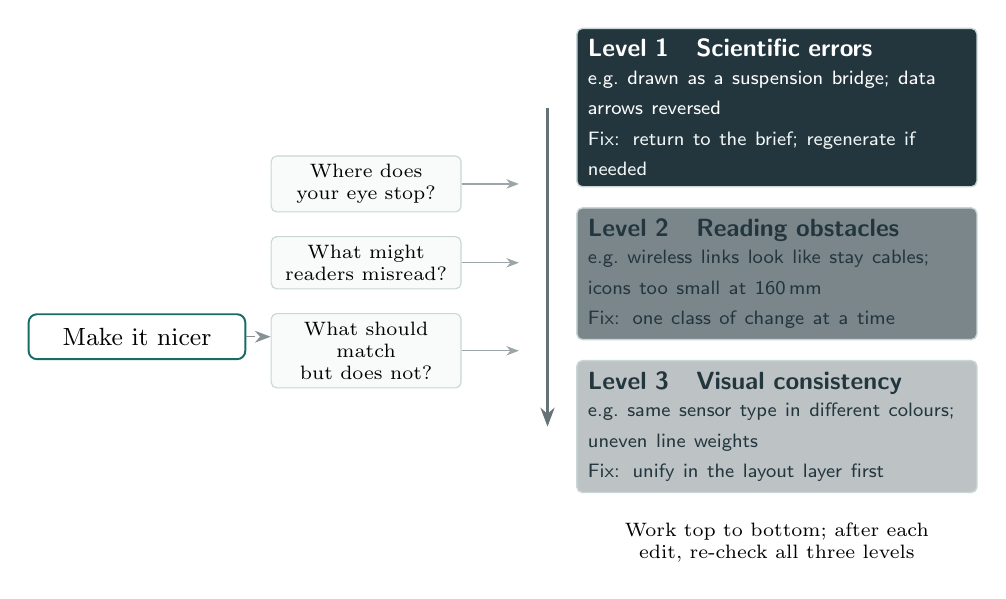
\begin{tikzpicture}[x=\linewidth/100,y=\linewidth/100]
\begin{scope}[
  font=\sffamily\small,
  level/.style={
    draw=BookRule, line width=0.5pt, rounded corners=2pt,
    minimum width=50mm, minimum height=15mm, align=left, inner sep=4pt,
    text width=48mm, anchor=west,
  },
  qbox/.style={
    draw=BookRule, fill=BookPale!40, rounded corners=2pt,
    align=center, inner sep=3pt, text width=22mm, font=\scriptsize,
  },
]
  \node[
    draw=BookTeal, line width=0.7pt, fill=white, rounded corners=3pt,
    align=center, inner sep=5pt, text width=24mm, font=\small,
  ] (bubble) at (8,42) {Make it nicer};
  \draw[BookInk!55, dashed, -{Stealth[length=2mm]}] (bubble.east) -- (22,42);

  \node[qbox] (q1) at (32,58) {Where does\\your eye stop?};
  \node[qbox, below=3mm of q1] (q2) {What might\\readers misread?};
  \node[qbox, below=3mm of q2] (q3) {What should match\\but does not?};

  \foreach \q in {q1,q2,q3} {
    \draw[BookInk!45, -{Stealth[length=1.6mm]}] (\q.east) -- ++(6,0);
  }

  \node[level, fill=BookInk, text=white] (L1) at (54,66) {%
    \textbf{Level 1\quad Scientific errors}\\[-1pt]
    {\scriptsize e.g.\ drawn as a suspension bridge; data arrows reversed}\\
    {\scriptsize\textcolor{BookPale!90}{Fix: return to the brief; regenerate if needed}}};
  \node[level, fill=BookInk!60, text=BookInk, below=2.5mm of L1] (L2) {%
    \textbf{Level 2\quad Reading obstacles}\\[-1pt]
    {\scriptsize e.g.\ wireless links look like stay cables; icons too small at 160\,mm}\\
    {\scriptsize Fix: one class of change at a time}};
  \node[level, fill=BookInk!30, text=BookInk, below=2.5mm of L2] (L3) {%
    \textbf{Level 3\quad Visual consistency}\\[-1pt]
    {\scriptsize e.g.\ same sensor type in different colours; uneven line weights}\\
    {\scriptsize Fix: unify in the layout layer first}};

  \coordinate (ordA) at ($(L1.west)+(-3,0)$);
  \coordinate (ordB) at ($(L3.west)+(-3,0)$);
  \draw[BookInk!70, line width=0.8pt, -{Stealth[length=2.4mm]}] (ordA) -- (ordB);
  \node[font=\scriptsize, align=center, text width=46mm, anchor=north]
    at ($(L3.south)+(0,-2.5mm)$) {Work top to bottom; after each edit, re-check all three levels};
\end{scope}
\end{tikzpicture}

\newpage
\section*{FIG ch11-07 ch07 collateral (zh)}
% FIG ch11-07 Chapter 7 collateral reuse (Chinese)
\usetikzlibrary{arrows.meta,calc}
\begin{tikzpicture}
  \def\panelW{0.31\linewidth}
  \definecolor{Ch11AnnotRed}{HTML}{C0392B}
  \node[anchor=south west, inner sep=0] (imA) at (0,0) {%
    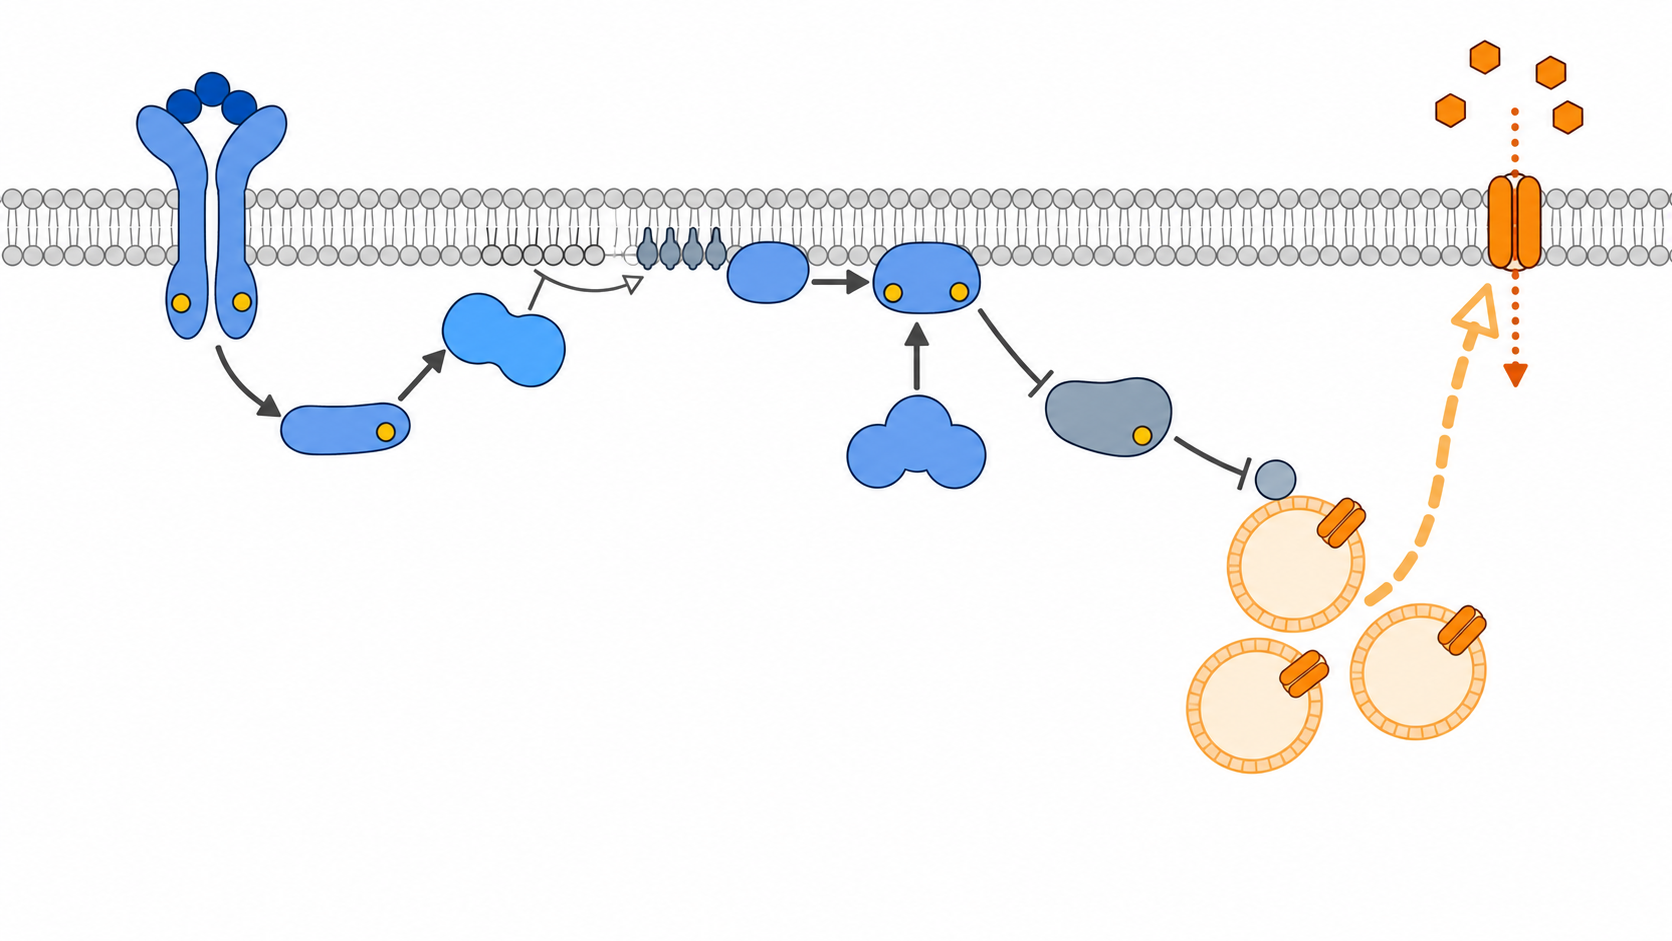
\includegraphics[width=\panelW]{figures/ch11/ch11-07a-ch07-v2.png}};
  \node[font=\small\sffamily, anchor=south] at ($(imA.north)+(0,2mm)$) {V2 基准};

  \node[anchor=south west, inner sep=0] (imB) at (0.345\linewidth,0) {%
    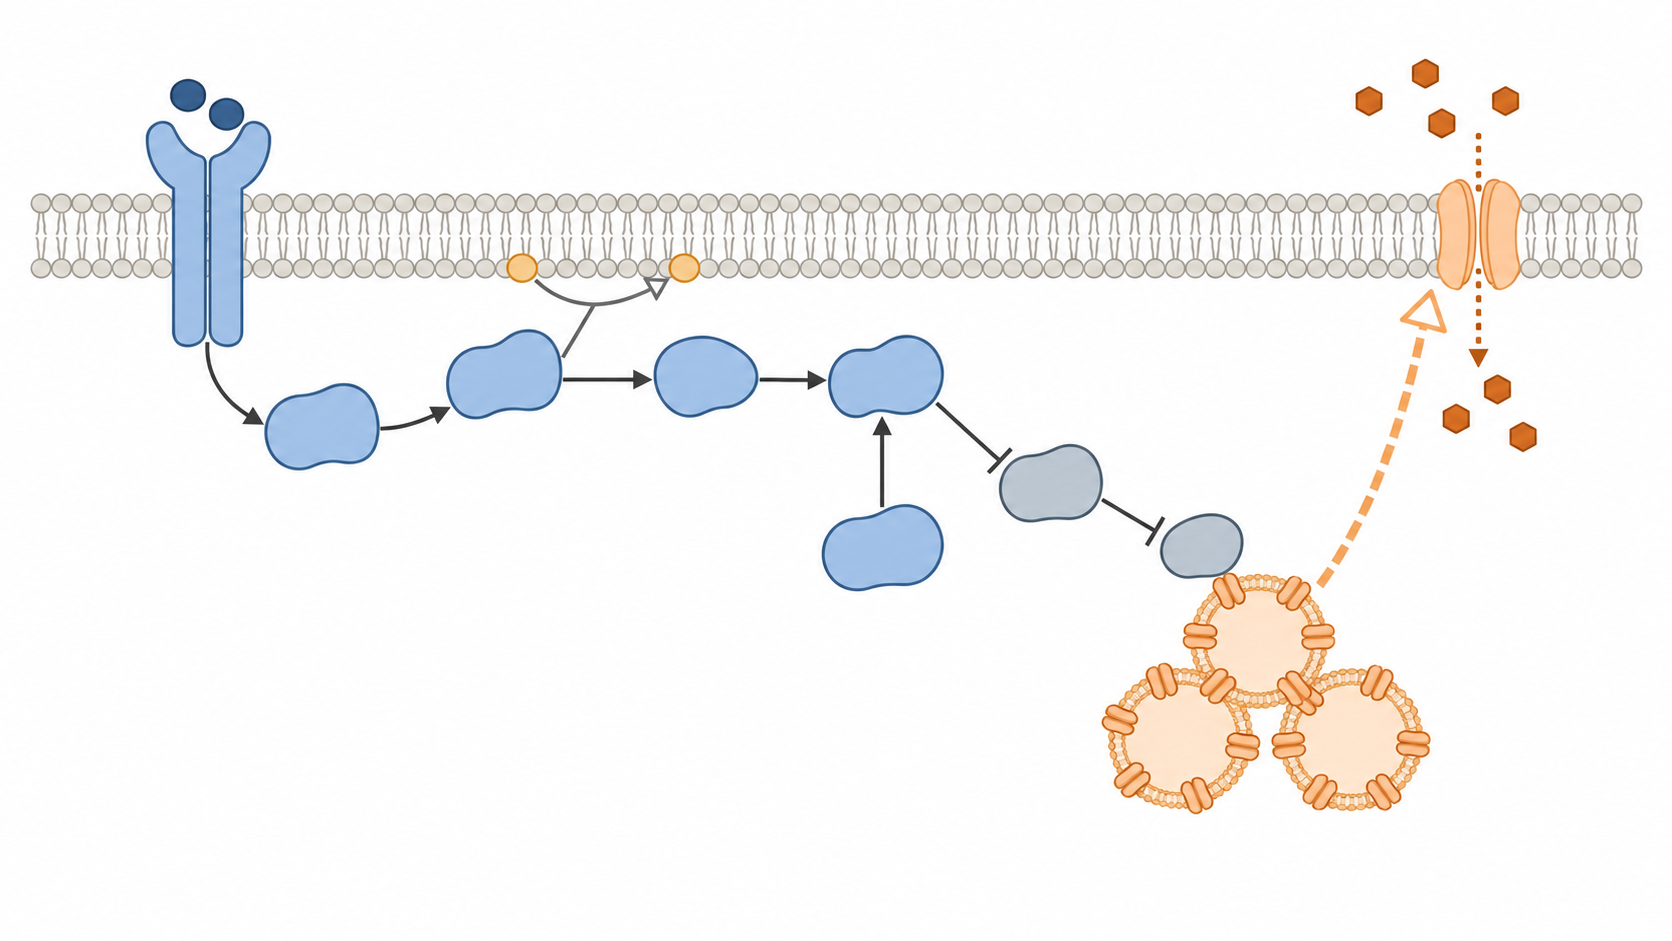
\includegraphics[width=\panelW]{figures/ch11/ch11-07b-ch07-v3-alt1.png}};
  \node[font=\small\sffamily, anchor=south] at ($(imB.north)+(0,2mm)$) {V3 第 1 次（不采用）};
  \begin{scope}[x={(imB.south east)},y={(imB.north west)}]
    \draw[Ch11AnnotRed, line width=0.7pt] (0.11,0.28) circle (0.035);
    \node[font=\scriptsize\sffamily, text=Ch11AnnotRed, anchor=west] at (0.15,0.28) {(a)};
    \draw[Ch11AnnotRed, line width=0.7pt] (0.10,0.08) circle (0.04);
    \node[font=\scriptsize\sffamily, text=Ch11AnnotRed, anchor=west] at (0.14,0.08) {(b)};
    \draw[Ch11AnnotRed, line width=0.7pt] (0.48,0.38) circle (0.06);
    \node[font=\scriptsize\sffamily, text=Ch11AnnotRed, anchor=west] at (0.54,0.38) {(c)};
    \draw[Ch11AnnotRed, line width=0.7pt] (0.34,0.36) circle (0.045);
    \node[font=\scriptsize\sffamily, text=Ch11AnnotRed, anchor=west] at (0.39,0.36) {(d)};
    \draw[Ch11AnnotRed, line width=0.7pt] (0.76,0.70) circle (0.07);
    \node[font=\scriptsize\sffamily, text=Ch11AnnotRed, anchor=west] at (0.82,0.70) {(e)};
  \end{scope}

  \node[anchor=south west, inner sep=0] (imC) at (0.69\linewidth,0) {%
    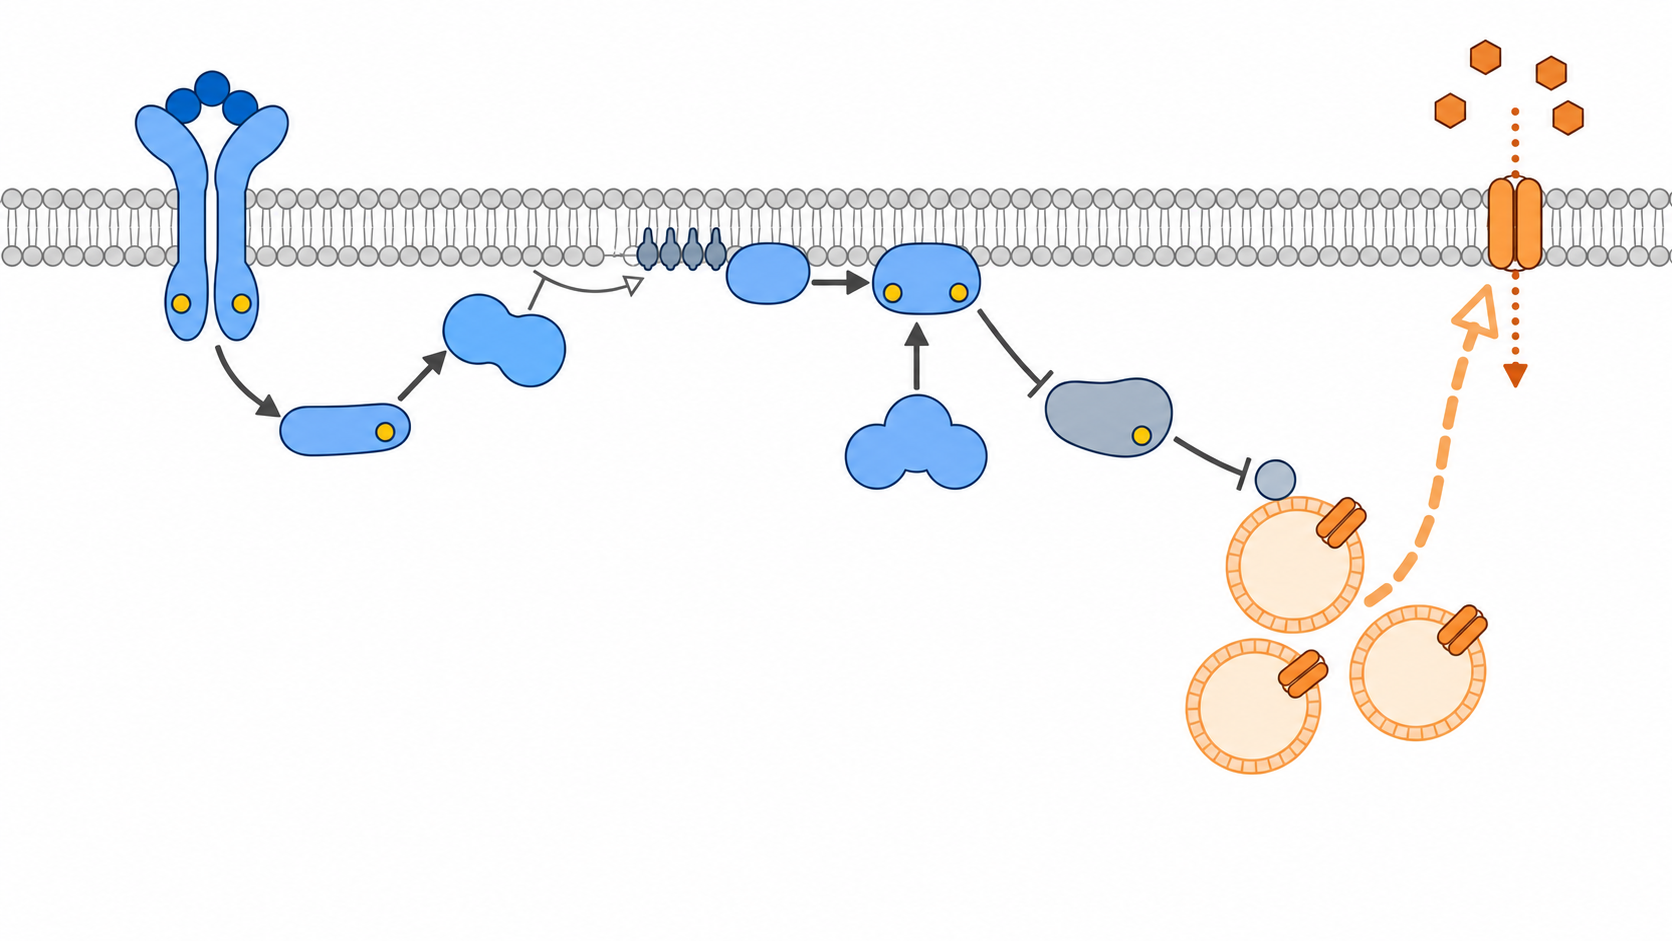
\includegraphics[width=\panelW]{figures/ch11/ch11-07c-ch07-v3.png}};
  \node[font=\small\sffamily, anchor=south] at ($(imC.north)+(0,2mm)$) {V3 第 2 次（采用）};
\end{tikzpicture}

\newpage
\section*{FIG ch11-07 ch07 collateral (en)}
% FIG ch11-07 Chapter 7 collateral reuse (English)
\usetikzlibrary{arrows.meta,calc}
\begin{tikzpicture}
  \def\panelW{0.31\linewidth}
  \definecolor{Ch11AnnotRed}{HTML}{C0392B}
  \node[anchor=south west, inner sep=0] (imA) at (0,0) {%
    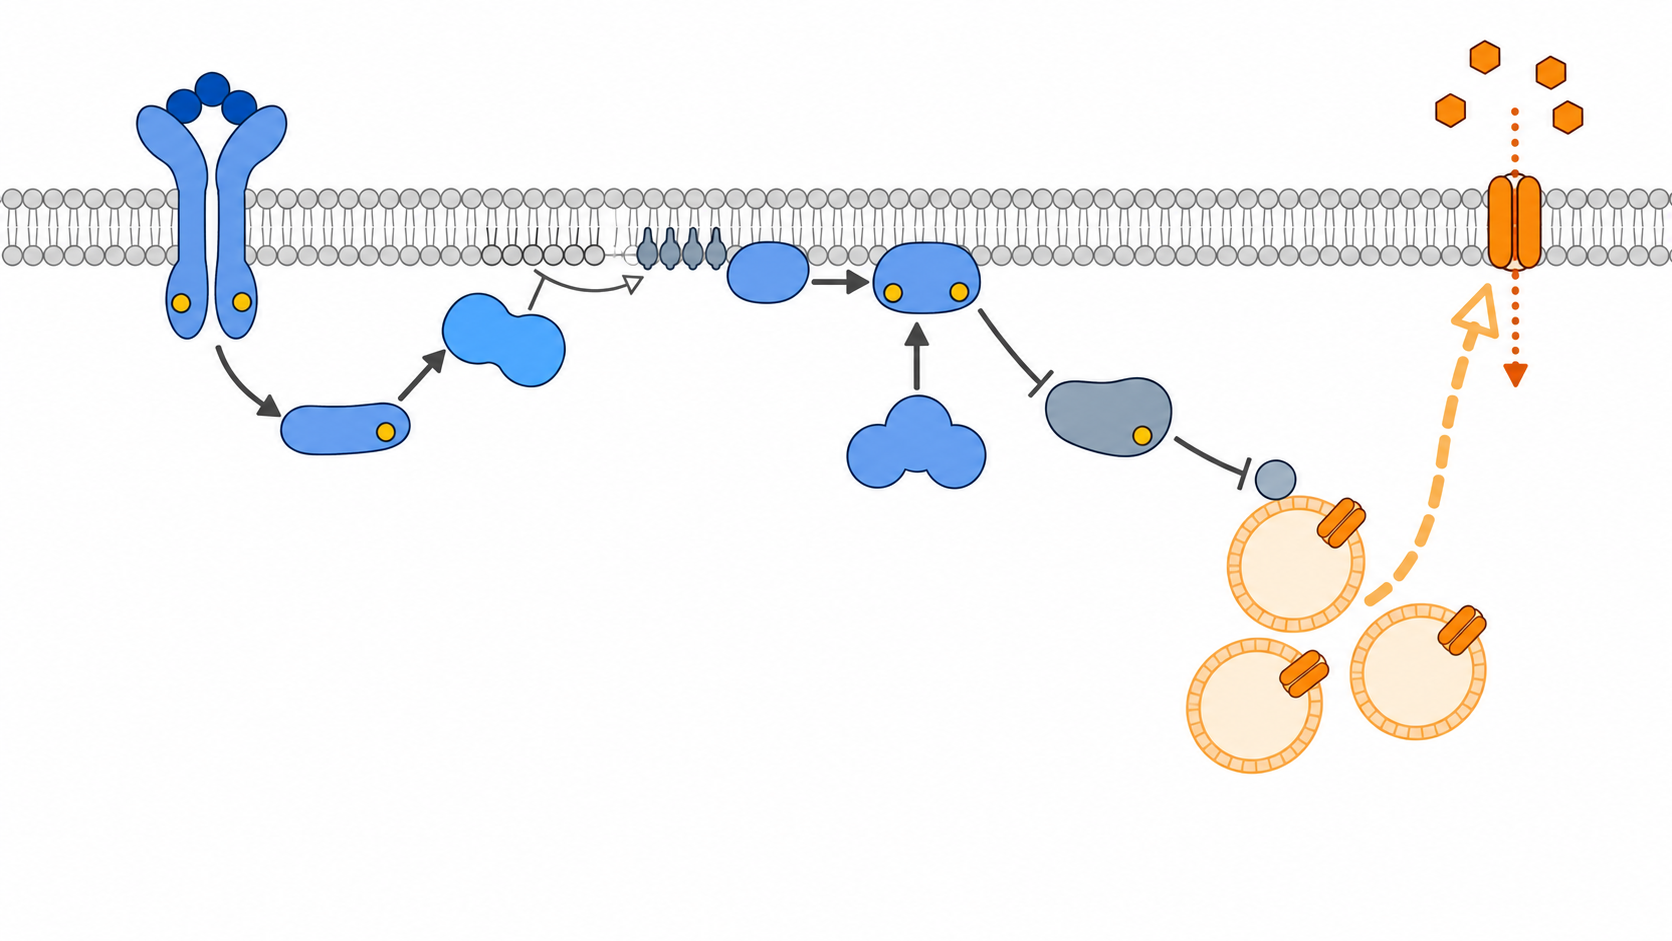
\includegraphics[width=\panelW]{figures/ch11/ch11-07a-ch07-v2.png}};
  \node[font=\small\sffamily, anchor=south] at ($(imA.north)+(0,2mm)$) {V2 baseline};

  \node[anchor=south west, inner sep=0] (imB) at (0.345\linewidth,0) {%
    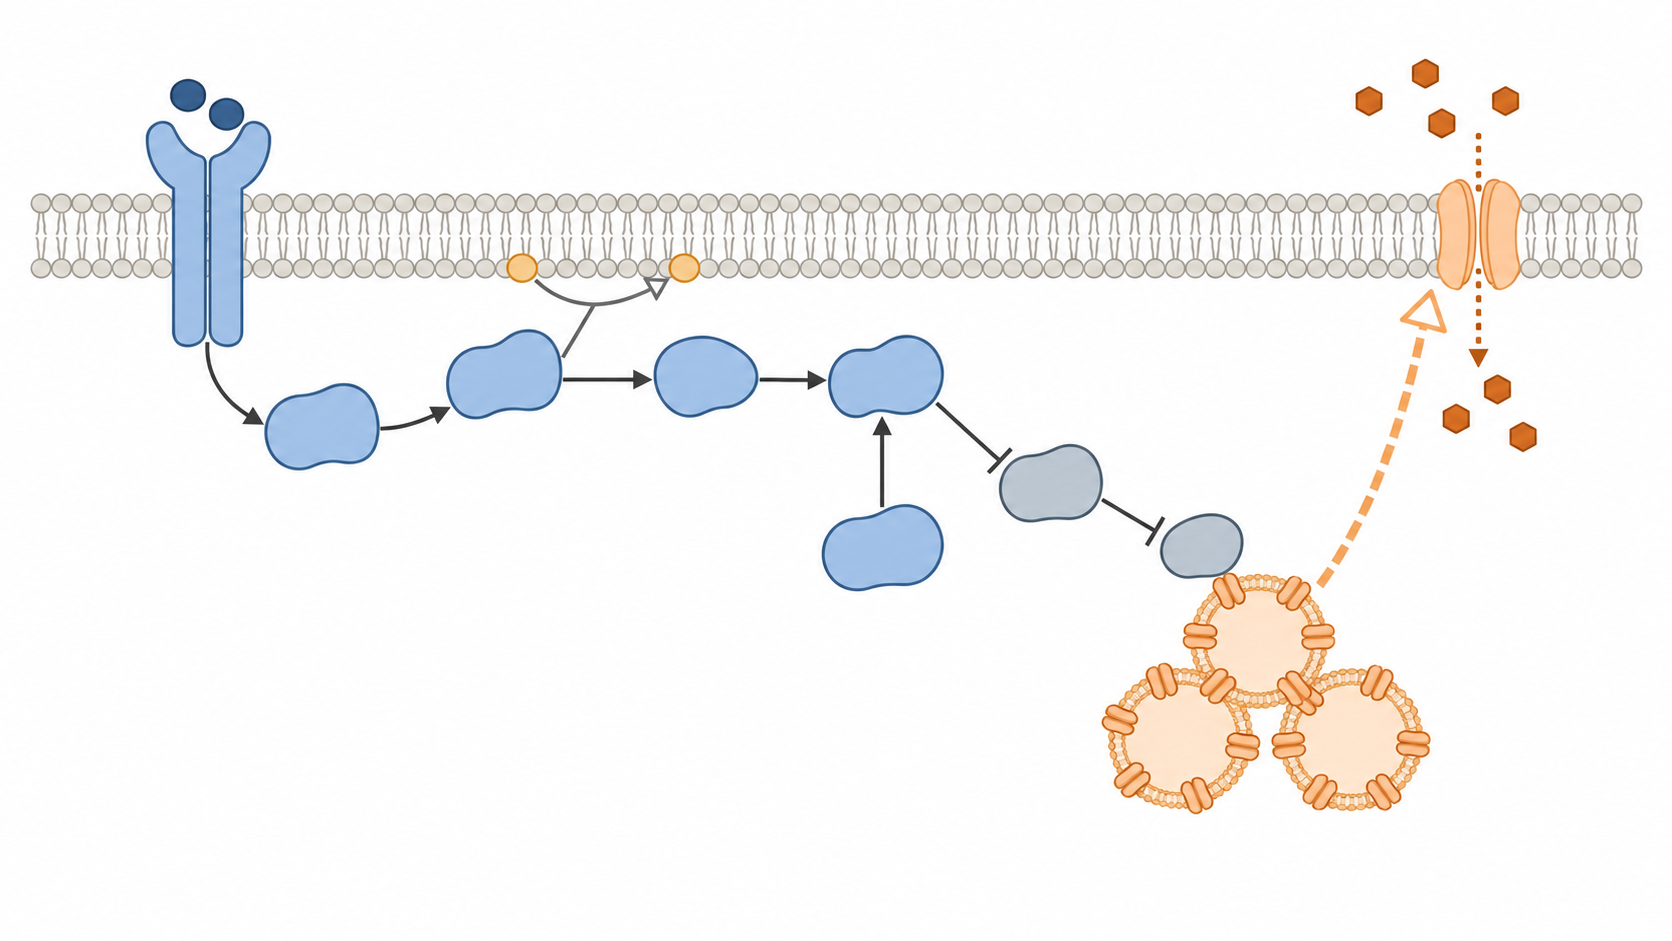
\includegraphics[width=\panelW]{figures/ch11/ch11-07b-ch07-v3-alt1.png}};
  \node[font=\small\sffamily, anchor=south] at ($(imB.north)+(0,2mm)$) {V3, attempt 1 (rejected)};
  \begin{scope}[x={(imB.south east)},y={(imB.north west)}]
    \draw[Ch11AnnotRed, line width=0.7pt] (0.11,0.28) circle (0.035);
    \node[font=\scriptsize\sffamily, text=Ch11AnnotRed, anchor=west] at (0.15,0.28) {(a)};
    \draw[Ch11AnnotRed, line width=0.7pt] (0.10,0.08) circle (0.04);
    \node[font=\scriptsize\sffamily, text=Ch11AnnotRed, anchor=west] at (0.14,0.08) {(b)};
    \draw[Ch11AnnotRed, line width=0.7pt] (0.48,0.38) circle (0.06);
    \node[font=\scriptsize\sffamily, text=Ch11AnnotRed, anchor=west] at (0.54,0.38) {(c)};
    \draw[Ch11AnnotRed, line width=0.7pt] (0.34,0.36) circle (0.045);
    \node[font=\scriptsize\sffamily, text=Ch11AnnotRed, anchor=west] at (0.39,0.36) {(d)};
    \draw[Ch11AnnotRed, line width=0.7pt] (0.76,0.70) circle (0.07);
    \node[font=\scriptsize\sffamily, text=Ch11AnnotRed, anchor=west] at (0.82,0.70) {(e)};
  \end{scope}

  \node[anchor=south west, inner sep=0] (imC) at (0.69\linewidth,0) {%
    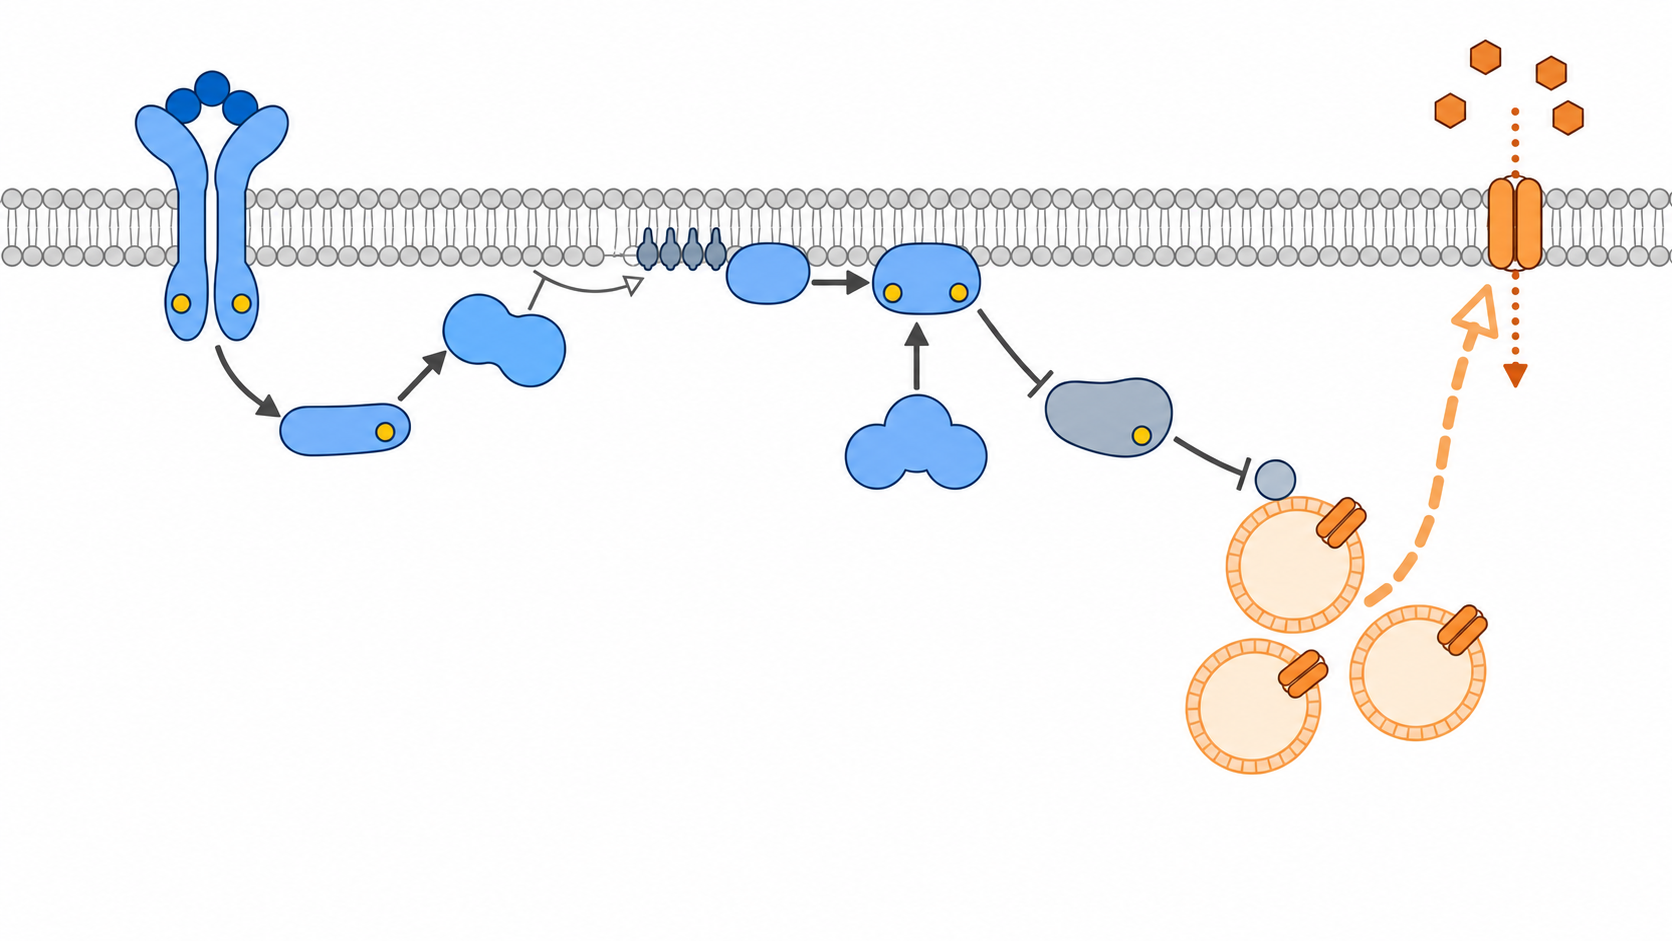
\includegraphics[width=\panelW]{figures/ch11/ch11-07c-ch07-v3.png}};
  \node[font=\small\sffamily, anchor=south] at ($(imC.north)+(0,2mm)$) {V3, attempt 2 (accepted)};
\end{tikzpicture}

\newpage
\section*{FIG ch11-08 version tree (zh)}
% FIG ch11-08 version tree (Chinese)
\usetikzlibrary{arrows.meta,positioning,fit,calc}
\definecolor{Ch11BadRed}{HTML}{C0392B}
\definecolor{Ch11GoodGreen}{HTML}{2E8B57}
\providecommand{\ChElevenThumb}[2]{%
  \IfFileExists{#1}{%
    \includegraphics[width=24mm]{#1}%
  }{%
    \fbox{\parbox[c][16mm][c]{24mm}{\centering\scriptsize\sffamily #2\\{\tiny （底图待出）}}}}%
}
\begin{tikzpicture}[
  x=1mm, y=1mm,
  font=\sffamily\footnotesize,
  edge/.style={draw=BookInk!60, -{Stealth[length=2mm]}, line width=0.55pt},
  badedge/.style={draw=Ch11BadRed!70, dashed, -{Stealth[length=2mm]}},
  nlabel/.style={align=center, text width=26mm, font=\scriptsize},
]
  \node (V1) at (0,0) {\ChElevenThumb{figures/ch11/ch11-02-v1-vague.png}{V1}};
  \node[nlabel, below=1mm of V1] {模糊提示词};

  \node (V2) [below=14mm of V1] {\ChElevenThumb{figures/ch11/ch11-03-v2-brief.png}{V2\\基准}};
  \node[nlabel, below=1mm of V2] {\textbf{结构基准}};

  \node (V3) [below=14mm of V2] {\ChElevenThumb{figures/ch11/ch11-04-v3-collateral.png}{V3}};
  \node[nlabel, below=1mm of V3, text=Ch11BadRed] {连带变化\\{\tiny（不采用）}};

  \node (V4) at (42,-28) {\ChElevenThumb{figures/ch11/ch11-06-v4-recovered.png}{V4}};
  \node[nlabel, below=1mm of V4, text=Ch11GoodGreen] {回到 V2\\只改无线线};

  \node (Final) at (84,-28) {\ChElevenThumb{figures/ch11/ch11-06-v4-recovered.png}{终稿}};
  \node[nlabel, below=1mm of Final] {TikZ 标签与图例};

  \draw[edge] (V1) -- node[left, font=\tiny, align=right] {重写\\输入} (V2);
  \draw[edge] (V2) -- node[right=1.5mm, font=\tiny, align=left] {只改\\无线线} (V3);
  \draw[edge] (V2.east) -- node[above, font=\tiny] {只改无线线\\+ 保留清单} (V4.west);
  \draw[edge] (V4.east) -- node[above, font=\tiny] {叠加标签\\与图例} (Final.west);

  \node[draw=Ch11BadRed, dashed, rounded corners=2pt, inner sep=4pt, fit=(V3)] {};
  \node[font=\scriptsize, text=Ch11BadRed, right=1mm of V3] {×};

  \node (Vp1) at (42,-66) {\fbox{\parbox[c][16mm][c]{24mm}{\centering\scriptsize V3$'$\\示意}}};
  \node[font=\tiny, below=1mm of Vp1, text width=28mm, align=center] {把消失的天线加回来};
  \node (Vp2) [right=12mm of Vp1] {\fbox{\parbox[c][16mm][c]{24mm}{\centering\scriptsize V3$''$\\示意}}};
  \node[font=\tiny, below=1mm of Vp2, text width=28mm, align=center] {又一处变化};
  \draw[badedge] (Vp1) -- (Vp2);
  \node[draw=BookInk!40, dashed, rounded corners=2pt, inner sep=6pt,
    fit=(Vp1)(Vp2), label={[font=\scriptsize, yshift=2mm]above:错误做法：在错误版本上叠加}] {};
  \draw[badedge] (V3.east) -- ++(6,0) |- (Vp1.west);
\end{tikzpicture}

\newpage
\section*{FIG ch11-08 version tree (en)}
% FIG ch11-08 version tree (English)
\usetikzlibrary{arrows.meta,positioning,fit,calc}
\definecolor{Ch11BadRed}{HTML}{C0392B}
\definecolor{Ch11GoodGreen}{HTML}{2E8B57}
\providecommand{\ChElevenThumb}[2]{%
  \IfFileExists{#1}{%
    \includegraphics[width=24mm]{#1}%
  }{%
    \fbox{\parbox[c][16mm][c]{24mm}{\centering\scriptsize\sffamily #2\\{\tiny (base pending)}}}}%
}
\begin{tikzpicture}[
  x=1mm, y=1mm,
  font=\sffamily\footnotesize,
  edge/.style={draw=BookInk!60, -{Stealth[length=2mm]}, line width=0.55pt},
  badedge/.style={draw=Ch11BadRed!70, dashed, -{Stealth[length=2mm]}},
  nlabel/.style={align=center, text width=26mm, font=\scriptsize},
]
  \node (V1) at (0,0) {\ChElevenThumb{figures/ch11/ch11-02-v1-vague.png}{V1}};
  \node[nlabel, below=1mm of V1] {One-line prompt};

  \node (V2) [below=14mm of V1] {\ChElevenThumb{figures/ch11/ch11-03-v2-brief.png}{V2\\baseline}};
  \node[nlabel, below=1mm of V2] {\textbf{Structural baseline}};

  \node (V3) [below=14mm of V2] {\ChElevenThumb{figures/ch11/ch11-04-v3-collateral.png}{V3}};
  \node[nlabel, below=1mm of V3, text=Ch11BadRed] {Collateral change\\{\tiny (rejected)}};

  \node (V4) at (42,-28) {\ChElevenThumb{figures/ch11/ch11-06-v4-recovered.png}{V4}};
  \node[nlabel, below=1mm of V4, text=Ch11GoodGreen] {Back to V2\\wireless lines only};

  \node (Final) at (84,-28) {\ChElevenThumb{figures/ch11/ch11-06-v4-recovered.png}{Final}};
  \node[nlabel, below=1mm of Final] {TikZ labels \& legend};

  \draw[edge] (V1) -- node[left, font=\tiny, align=right] {Rewrite\\input} (V2);
  \draw[edge] (V2) -- node[right=1.5mm, font=\tiny, align=left] {Wireless\\lines only} (V3);
  \draw[edge] (V2.east) -- node[above, font=\tiny] {Wireless +\\keep list} (V4.west);
  \draw[edge] (V4.east) -- node[above, font=\tiny] {Labels \&\\legend} (Final.west);

  \node[draw=Ch11BadRed, dashed, rounded corners=2pt, inner sep=4pt, fit=(V3)] {};
  \node[font=\scriptsize, text=Ch11BadRed, right=1mm of V3] {×};

  \node (Vp1) at (42,-66) {\fbox{\parbox[c][16mm][c]{24mm}{\centering\scriptsize V3$'$\\schematic}}};
  \node[font=\tiny, below=1mm of Vp1, text width=28mm, align=center] {Add back missing antenna};
  \node (Vp2) [right=12mm of Vp1] {\fbox{\parbox[c][16mm][c]{24mm}{\centering\scriptsize V3$''$\\schematic}}};
  \node[font=\tiny, below=1mm of Vp2, text width=28mm, align=center] {Another drift};
  \draw[badedge] (Vp1) -- (Vp2);
  \node[draw=BookInk!40, dashed, rounded corners=2pt, inner sep=6pt,
    fit=(Vp1)(Vp2), label={[font=\scriptsize, yshift=2mm]above:Wrong: patch the faulty version}] {};
  \draw[badedge] (V3.east) -- ++(6,0) |- (Vp1.west);
\end{tikzpicture}

\end{document}
